\documentclass{report}
\usepackage[T1]{fontenc} % Fontes T1
\usepackage[utf8]{inputenc} % Input UTF8
\usepackage[backend=biber, style=ieee]{biblatex} % para usar bibliografia
\usepackage{csquotes}
\usepackage[portuguese]{babel} %Usar língua portuguesa
\usepackage{blindtext} % Gerar texto automaticamente
\usepackage[printonlyused]{acronym}
\usepackage{hyperref} % para autoref
\usepackage{graphicx}
\graphicspath{ {./imagesbac/} }
\graphicspath{ {./imagescodebac/} }
\graphicspath{ {./images sql/} }
\graphicspath{ {./lfi/} }
\usepackage{caption}
\usepackage{subcaption}


\bibliography{bibliografia}


\begin{document}
%%
% Definições
%
\def\titulo{Vulnerabilidades WEB}
\def\data{19/12/2021}
\def\autores{André Miragaia, André Cruz}
\def\autorescontactos{(108412) andre.miragaia@ua.pt, (110554) afgc@ua.pt}
\def\versao{VERSAO}
\def\departamento{DETI}
\def\empresa{UA}
\def\logotipo{ua.pdf}
%
%%%%%% CAPA %%%%%%
%
\begin{titlepage}

\begin{center}
%
\vspace*{50mm}
%
{\Huge \titulo}\\ 
%
\vspace{10mm}
%
{\Large \empresa}\\
%
\vspace{10mm}
%
{\LARGE \autores}\\ 
%
\vspace{30mm}
%
\begin{figure}[h]
\center
\includegraphics{\logotipo}
\end{figure}
%
\vspace{30mm}
\end{center}
%
\begin{flushright}
\end{flushright}
\end{titlepage}

%%  Página de Título %%
\title{%
{\Huge\textbf{\titulo}}\\
{\Large \departamento\\ \empresa}
}
%
\author{%
    \autores \\
    \autorescontactos
}
%
\date{\data}
%
\maketitle

\pagenumbering{roman}

%%%%%% RESUMO %%%%%%
\begin{abstract}
Num mundo cada vez mais digital todos nós acessamos vários sistemas web no nosso dia a dia, usando vários tipos de dispositivo para nos conectarmos (smartphone, computador, tablet, smartwatch, etc). Mas ao termos um mundo mais conectado não só temos o dever de criar aplicações web funcionais mas também garantir a segurança de todos os que vão usá-las.

 trabalho vai ao encontro do tema pois tem como objetivo nos instruir sobre as vulnerabilidades mais comuns na web, as consequências de cada e como as corrigir de forma a tornarmos o mundo digital num lugar mais seguro para todos e evitar situações extremamente inconvenientes que poderiam ser evitadas de maneira simples se forem tomadas as devidas precauções.

Nos capítulos subsequentes iremos apresentar pedaços de código incompletos para analisarmos e para percebermos o que faz as vulnerabilidades existirem e as possíveis soluções para cada, iremos também criar cenários para cada vulnerabilidade não só para ser perceptível a gravidade de cada uma das mesmas, mas também para percebermos como uma pessoa mal intencionada pode as usar em seu proveito.

As vulnerabilidades que escolhemos têm como base a OWASP, uma comunidade que além de ter um trabalho crucial no campo da cibersegurança, também disponibilizam todos os anos as vulnerabilidades mais recorrentes divididas em catalogos.
\end{abstract}

%%%%%%% Agradecimentos %%%%%%
%% Segundo glisc deveria aparecer após conclusão...
%\renewcommand{\abstractname}{Agradecimentos}
%\begin{abstract}
%Eventuais agradecimentos.
%Comentar bloco caso não existam agradecimentos a fazer.
%\end{abstract}


\tableofcontents
% \listoftables     % descomentar se necessário
% \listoffigures    % descomentar se necessário


%%%%%%%%%%%%%%%%%%%%%%%%%%%%%%%
\clearpage
\pagenumbering{arabic}

%%%%%%%%%%%%%%%%%%%%%%%%%%%%%%%%
\chapter{Introdução}
\label{chap.introducao}

%%%%%%%%%%USAR AUTOREFS%%%%%%
Levando em conta o desenvolvimento do mundo digital nos dias de hoje quer em termos de numero de utilizadores quer na complexidade do mesmo, julgamos pertinente abordar a parte da segurança no que toca a este mundo. Foram escolhidos dois catálogos de vulnerabilidades web que devido á falta de informação revelada pelos utilizadores, são cada vez mais comuns o que aumenta as chances de trazer uma má experiência ao utilizador prejudicando o mesmo diretamente em varias frentes. Estas vulnerabilidades vão ser explicitadas com exemplos e informação pertinente, com a revelação de medidas de prevenção para exista pelo menos uma chance menor do utilizador ser exposto.

O conteúdo vai ser dividido em seis capítulos, Introdução, Metodologia, Vulnerabilidades Broken Access Control, Vulnerabilidades de Injeção, Análise, Conclusões.
\chapter{Metodologia}
\label{chap.metodologia}
Para a obtenção de resultados foram exploradas 2 dos 10 catálogos de  vulnerabilidades mais comuns no ano de 2021, em cada uma delas foi feita uma descrição geral e as consequências que as mesmas podem trazer para quem está exposto. 

Foram apresentados exemplos significativos de situações realistas aonde as mesmas estão presentes identificando quais seriam as medidas necessárias a tomar para evitar as mesmas. Para fins demonstrativos foram também apresentadas imagens e partes de código exemplo para explicitar efetivamente como é que cada vulnerabilidade se desenvolve na pratica.

%\section{Exemplos}

%\subsection{Utilização de acrónimos}
%Esta é a primeira invocação do acrónimo \ac{ua}.
%E esta é a segunda: \ac{ua}.

%Outras duas referências a \ac{miect}
%e \ac{miect}.
%TEMOS DE ALTERAR OS ACRONIMOS NO FINAL%
%\subsection{Referências bibliográficas}
%Informação relativa à estrutura formal de um relatório pode ser obtida
%na página do \ac{glisc}\cite{glisc}.

\chapter{ Broken Access Control}
\clearpage
\label{chap.bac}
\section{Descrição geral}

Esta é uma vulnerabilidade que tem vindo a crescer ao longo do tempo, em 2020 esteve na quinta posição na lista das 10 vulnerabilidades mais comuns, feita pela OWASP tendo subido para a primeira posição em 2021 com uma testagem equivalente a 94\% das aplicações para alguma forma de "\ac{bac}" com uma taxa de incidência de 3,81\%.\cite{owasptop10}

O Access Control faz com que os utilizadores não possam agir fora das permissões pretendidas, geralmente as falhas levam à divulgação, modificação ou até mesmo destruição de informações não autorizadas de todos os dados, ou ao desempenho de uma função comercial fora dos limites do utilizador.

As vulnerabilidades mais comuns de \ac{bac} incluem:
\begin{list}{--}{}
    \item Burlar a verificação de Access Control modificando a URL, o estado interno da aplicação, a página HTML ou usando uma ferramenta para fazer ataques personalizados na API.
    \item Alterando a chave primária para a de outro utilizador podendo assim visualizar ou fazer alterações na conta do mesmo.
    \item Elevação de privilégios podendo atuar com um utilizador sem estar logado ou atuar como administrador estando logado como um utilizador padrão.
    \item Manipulação de metadados, adulterando ou reproduzindo um token de controlo de acesso \ac{jwt}, um cookie ou manipulando um campo oculto para elevar privilégios, ou abusando da falta de validação de \ac{jwt}.
    \item Abusar da configuração incorreta do CORS permitindo assim acessos não autorizados à API.
    \item Forçar a navegação para paginas autenticadas através de um utilizador não autenticado ou para paginas privilegiadas através de um utilizador padrão abusando da falta de verificação para os métodos POST, PUT e DELETE.
\end{list}
\clearpage
\section{Falta de verificação da informação}
\subsection{Descrição geral e consequências}

O fator mais comum que possibilita a existência de vulnerabilidades relacionadas a \ac{bac} é a falta de verificação, o que abre a porta para utilizadores não autorizados terem acesso a informações sensíveis ou, em alguns casos, ter acesso a páginas que não deveriam ter acesso sem cumprir determinados requisitos como por exemplo acessar informações de outros utilizadores sem estar sequer logado o que pode ser bastante perigoso visto que os utilizadores com as permissões mais elevadas normalmente conseguem fazer alterações bastante sensíveis como alterar as páginas do servidor, criar páginas novas, entre outras coisas que podem comprometer bastante a segurança de todos. Agora vamos expor como a falta de verificação da informação pode ser bastante comprometedora.
\clearpage
\subsection{Código exemplo}	

Para ilustrar esta vulnerabilidade decidimos criar três arquivos, um chamado index.php, outro chamado conta.php e por ultimo um arquivo chamado robots.txt. O index.php é uma pagina de login que quando um utilizador é logado, este é redirecionado para a conta.php que irá exibir as informações desse utilizador. Já o robots.txt é um arquivo que tem como finalidade comunicar aos motores de busca (Google, Bing, etc) quais arquivos não queremos que sejam acessados, ou seja, se alguém pesquisou no google o nosso website, para evitar que apareça arquivos sensíveis nós colocamos no robots.txt os arquivos que não queremos que sejam exibidos.

\begin{figure}[!htb]
\minipage{0.70\textwidth}
  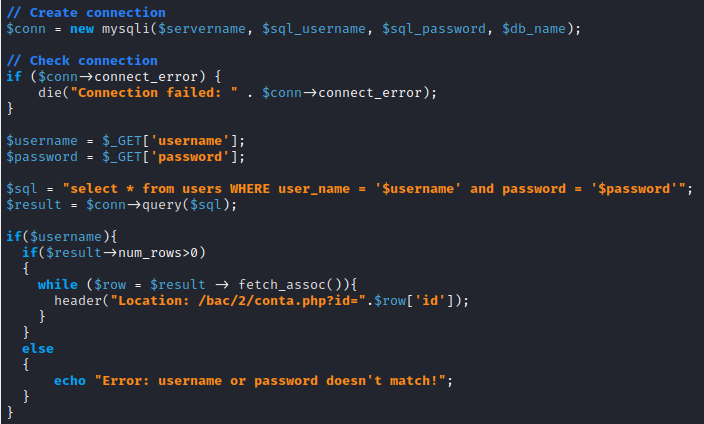
\includegraphics[width=\linewidth]{imagescodebac/baccode1.png}
  \caption{Sintaxe do index.php}\label{fig:index.php}
\endminipage\hfill
\minipage{0.30\textwidth}
  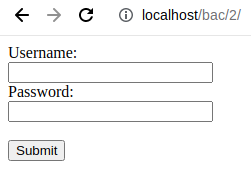
\includegraphics[width=\linewidth]{imagesbac/bac1.png}
  \caption{index.php}\label{fig:intefacelogin}
\endminipage
\end{figure}
\begin{figure}[!htb]
\minipage{0.70\textwidth}
  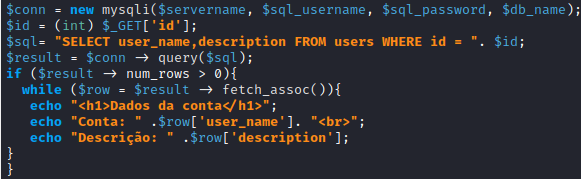
\includegraphics[width=\linewidth]{imagescodebac/baccode2.png}
  \caption{Sintaxe da conta.php}\label{fig:conta.php}
\endminipage\hfill
\minipage{0.30\textwidth}
  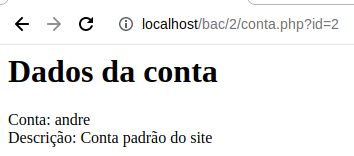
\includegraphics[width=\linewidth]{imagesbac/bac2.png}
  \caption{conta.php}\label{fig:userinfo}
\endminipage
\end{figure}
\clearpage
\subsection{Análise da sintaxe}	
	
Vamos começar por analisar o index.php. A variável \$conn vai criar uma conexão com a base de dados em que as variaveis \$servername, \$sql\textunderscore username, \$sql\textunderscore password e a \$db\textunderscore name armazenam, respetivamente, o ip do servidor onde esta a base de dados, o utilizador, a password e o nome da base de dados. Depois da variável \$conn, o "if" vai tentar se conectar com o banco de dados. Já as variáveis \$username e \$password vão receber o que o utilizador digitar. A seguir temos a variável \$sql que seleciona tudo o que está dentro da tabela users e compara se a variável \$username está dentro da coluna user\textunderscore name e se a \$password está dentro da coluna password. 

Logo depois temos a variável \$result que vai executar a variável \$sql, ou seja, vai fazer uma consulta na base de dados e procurar as informações que pedimos. A seguir temos um "if" que será executado quando o parâmetro "username" receber alguma coisa e logo a seguir será executado outro "if" caso o "número de linhas" recebidas pela variável \$result seja maior que zero. Dentro desse "if" temos um while que será executado enquanto todos valores extraídos da base de dados não forem lidos, esses valores serão armazenados numa variável chamada \$row. Por último temos a função header que vai redirecionar o utilizador para o arquivo conta.php com o "id" associado há conta do utilizador.

Agora vamos analisar a conta.php. A variável \$conn fará uma conexão com a base de dados, já a variável \$id vai armazenar o parâmetro "id" que foi enviado pelo index.php e a variável \$sql vai procurar o username e a descrição associados ao "id" que depois será executado pela variável \$result. Depois temos um "if" que vai verificar se o "número de linhas" é maior que zero e dentro dele temos um while que será executado enquanto todos os valores não forem lidos em que os mesmos serão armazenados numa variável chamada \$row. Por último temos as instruções echo que vão exibir os dados extraídos da base de dados, ou seja, o respetivo username e a sua descrição.

O grande problema desta sintaxe é que as informações são passadas diretamente pela URL sem qualquer tipo de verificação o que faz com que qualquer um possa modificar da forma que quer.
\clearpage
\subsection{Cenários de ataque}

\subsubsection{Primeiro cenário - Acessando outros utilizadores modificando o id da URL}

Neste cenário o atacante está logado numa conta chamada "andre" cujo "id" da conta é "2", ao mudarmos o "id" para outro valor, por exemplo para o valor "1", o que vai acontecer é que devido há falta de verificação o atacante consegue mudar para outra conta. Ao mudar o id para "1" o mesmo consegue ter acesso há conta "admin" que é a conta de administrador do website.

\begin{figure}[h]
 \centering
 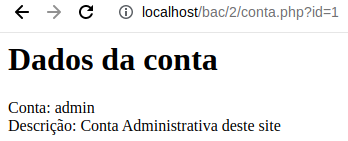
\includegraphics[scale=0.3]{imagesbac/bac3.png}
 \caption{Dados da Conta}
\end{figure}

\subsubsection{Segundo cenário - Acessando outros utilizadores sem estar logado}

Neste cenário o atacante não tem nenhuma conta no servidor e por isso a primeira coisa que ele vai fazer é procurar informações para poder realizar o seu propósito. 

Para isso ele vai entrar no arquivo robots.txt para procurar arquivos sensíveis. Ao entrar no robots.txt ele descobre que existe um arquivo chamado conta.php mas ao entrar no mesmo se depara com uma página em branco visto que não há nenhum parâmetro. Para encontrar os parâmetros ele vai usar uma ferramenta chamada Arjun programada em python que foi feita com esse propósito. Como podem ver o Arjun encontrou o parametro "id" e como o parâmetro só recebe números inteiros ele vai testar o valor "1" que por padrão é o do administrador na maioria dos servidores.
\cite{arjumgit}
\begin{figure}[!htb]
\minipage{0.30\textwidth}
  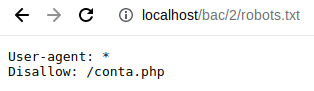
\includegraphics[width=\linewidth]{imagesbac/bac4.png}
  \caption{robots.txt}\label{fig:robots}
\endminipage\hfill
\minipage{0.40\textwidth}
  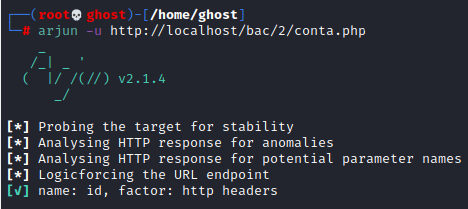
\includegraphics[width=\linewidth]{imagesbac/bac5.png}
  \caption{Arjun}\label{fig:arjun}
\endminipage\hfill
\minipage{0.30\textwidth}%
  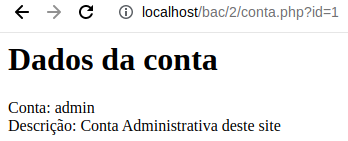
\includegraphics[width=\linewidth]{imagesbac/bac6.png}
  \caption{Interface admin}\label{fig:iadmin}
\endminipage
\end{figure}

\clearpage

\subsection{Como prevenir}
Nos cenários de ataque que apresentamos podemos concluir que este tipo de vulnerabilidade pode muito bem ser evitado simplesmente enviando as informações de uma pagina para a outra e depois verificando se há alguma alteração feita pelo utilizador no parâmetro "id". 

Para fazer essa verificação vamos acrescentar uma função presente no php chamada session\textunderscore start() que tem como objetivo criar uma sessão onde serão armazenados o username, a password e o id. 

Quando logado este será redirecionado para conta.php mas se o mesmo tentar mudar o id, o primeiro if que foi acrescentado fará com que seja redirecionado para a index.php mas caso o mesmo tente acessar a conta.php sem estar logado o segundo "if" que foi acrescentado fará com que seja redirecionado para o index.php e assim resolvemos o problema!

\begin{figure}[!htb]
\centering
\minipage{0.75\textwidth}
  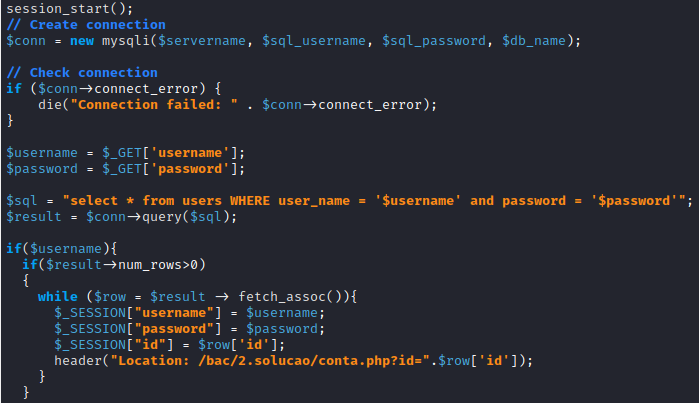
\includegraphics[width=\linewidth]{imagescodebac/baccode3.png}
  \caption{index.php}\label{fig:index.php}
\endminipage
\end{figure}
\begin{figure}[!htb]
\centering
\minipage{0.75\textwidth}
  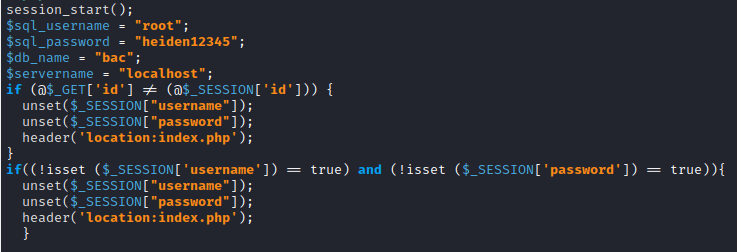
\includegraphics[width=\linewidth]{imagescodebac/baccode4.png}
  \caption{conta.php}\label{fig:conta.php}
\endminipage
\end{figure}


\clearpage
\section{Local File Inclusion}

	\subsection{Descrição geral e consequências}

O \ac{lfi} é uma vulnerabilidade que permite ao atacante ler arquivos dentro do servidor sem a permissão do mesmo. Este tipo de vulnerabilidade pode parecer bastante inofenciva mas na realidade não é visto que o atacante pode usar a mesma para ler arquivos importantes como o web.config, o passwd, o id\textunderscore rsa (SSH), arquivos de log, as páginas do servidor, etc sem contar que em alguns casos é possível a execução de código malicioso mas, felizmente este tipo de casos são bastante raros.
\cite{neuralegionlfi}
\cite{lfitesting}
	\subsection{Código exemplo}

Para ilustrar a vulnerabilidade decidimos criar um arquivo chamado fic.php em que o objetivo desta página é ler o index.php através do parâmetro "fic", usando o método GET.
Por exemplo:
http://127.0.0.1/bac/3/fic.php?fic=index.php

\begin{figure}[!htb]
\centering
\minipage{0.27\textwidth}
  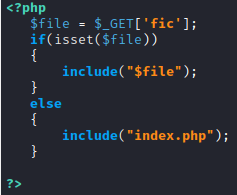
\includegraphics[width=\linewidth]{imagescodebac/baccode5.png}
  \caption{fic.php}\label{fig:fic.php}
\endminipage\hfill
\minipage{0.55\textwidth}
  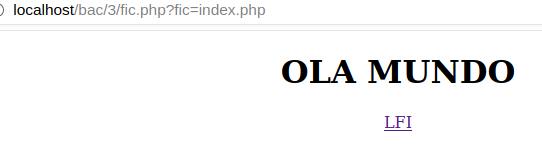
\includegraphics[width=\linewidth]{lfi/lfi1.png}}
  \caption{index.php}\label{fig:awesome_image3}
\endminipage
\end{figure}

	\subsection{Análise da sintaxe}

A variável \$file vai armazenar o que está no parâmetro "fic" e depois será executado o "if". Quando o "if" é executado, caso exista o parâmetro "fic" este será exibido na página, caso não exista a pagina irá exibir o index.php. Como já referimos antes, o problema deste tipo de vulnerabilidade é a falta de verificação e por isso qualquer um pode alterar o parâmetro "fic" para ler outros arquivos dentro do servidor.
\clearpage
	\subsection{Cenário de ataque - Invasão através do protocolo SSH}
 
Neste cenário o atacante tem como objetivo acessar o servidor através do protocolo SSH. Para isso, ele altera o parâmetro "fic", e coloca o diretório "/etc/passwd".
Como podemos ver existe um utilizador chamado "ghost". Agora o próximo passo é alterar o parâmetro e colocar o diretorio "/home/ghost/.ssh/id\textunderscore rsa".

\begin{figure}[!htb]
\centering
\minipage{0.70\textwidth}
  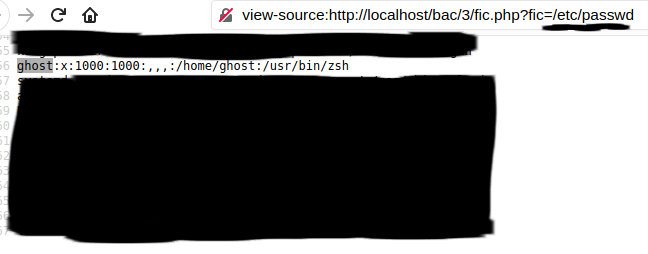
\includegraphics[width=\linewidth]{lfi/lfi2.png}
  \caption{/etc/passwd}\label{fig:passwd}
\endminipage
\end{figure}

Agora que o atacante sabe qual é o id\textunderscore rsa ele tem que simplesmente fazer um ataque bruteforce para descriptografar o id\textunderscore rsa e assim terá acesso ao servidor através do protocolo SSH.

\begin{figure}[!htb]
\centering
\minipage{0.80\textwidth}
  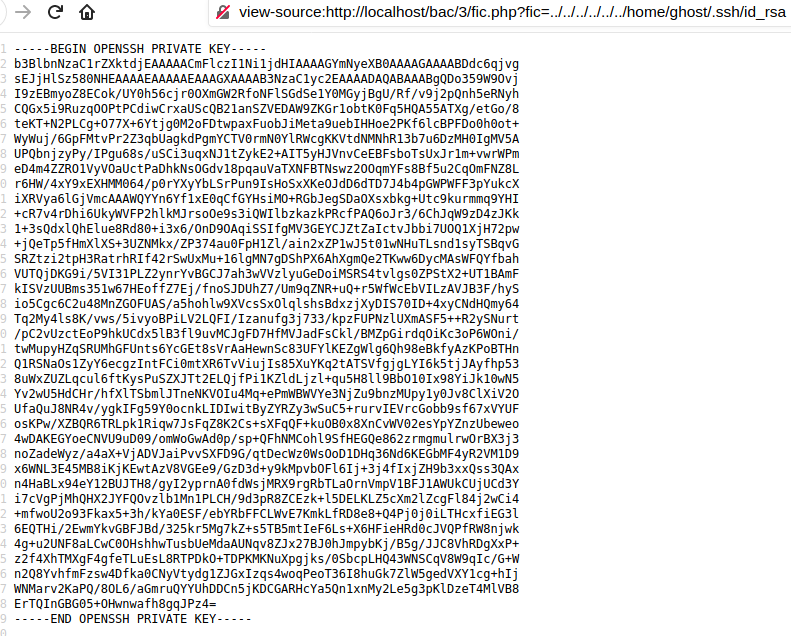
\includegraphics[width=\linewidth]{lfi/lfi3.png}
  \caption{id\textunderscore rsa}\label{fig:id_rsa}
\endminipage
\end{figure}
	\subsection{Como prevenir}

A forma mais comum de corrigir o \ac{lfi} é fazer uma lista de quais arquivos o parâmetro "fic" pode ter acesso e dependendo do caso o melhor seria atribuir um "id" a cada, para não exibir o nome ou o diretório. Alguns programadores preferem armazenar a lista na base de dados, mas não é a única forma. Por exemplo, neste caso a forma mais fácil e prática seria colocar no "if"  quais arquivos podem ser lidos e, caso tentem acessar outros, será exibido o index.php por padrão mas caso haja muitos arquivos o melhor seria armazenar numa base de dados.

 \begin{figure}[h]
 \centering
 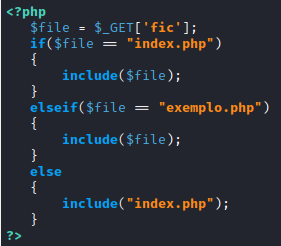
\includegraphics[scale=0.5]{imagescodebac/baccode6.png}
 \caption{fic.php}\label{fig:fic.php}
\end{figure}  


\chapter{Vulnerabilidades de Injeção}
\clearpage
\label{chap.injection}

\section{Descrição geral}

Os ataques por injeção apesar de estarem na 3ª posição no catálogo de vulnerabilidades reunidos pela OWASP em 2021,julgamos pertinente falar sobre elas pois além de serem muito frequentes com uma taxa máxima de incidência de 19.09\% também são as vulnerabilidades mais procuradas por hackers devido à quantidade de informação que os mesmos conseguem extrair através delas sem contar que em alguns casos também é possivel acessar arquivos, executar comandos, alterar a base de dados, entre outras opções. Por ser um catálogo com várias vulnerabilidades de injeção nós decidimos escolher o \ac{sqli}, o \ac{xss} e o OS Command Injection mas também existem outras como por exemplo o Carriage Return and Line Feed Injection (CRLF Injection) e o Lightweight Directory Access Protocol Injection (LDAP Injection).

	
\clearpage
\section{SQL Injection}
\subsection{Descrição geral e consequências}
	

O \ac{sqli} é uma vulnerabilidade que nos permite executar instruções SQL dentro de um sistema. O atacante que explora essa vulnerabilidade tem acesso total à base de dados podendo visualizar tudo o que está dentro dela incluído os utilizadores e as passwords armazenados mas além disso também pode modificar a base de dados e em alguns casos também pode fazer upload de arquivos para dentro do sistema o que torna uma das vulnerabilidades mais perigosas já descobertas. 

Esta vulnerabilidade é tão recorrente que já foi encontrada em sites do governo e de grandes empresas como foi o caso do governo da Turquia, da tesla em 2014 e da cisco em 2018. O \ac{sqli} pode afetar qualquer website que use uma base de dados como o MySQL, SQL Server entre outros mas o conceito por trás e sempre o mesmo. 
\clearpage
\subsection{Código exemplo}

Para ilustrar a vulnerabilidade decidimos usar como base uma pagina de login que acessa uma base de dados onde estão armazenadas os utilizadores e as passwords. A página principal, index.php, irá fazer uma requisição do tipo GET a um outro arquivo chamado vuln.php, que irá validar se o utilizador e a password introduzidos estão na base de dados. O método GET é um tipo de requisição que usa o formulário da página web para passar as informações diretamente pela URL, separando-as com um ponto de interrogação.
Exemplo:
http://127.0.0.1/vuln.php?username=andre\&password=p4ssw0rd.
Agora vamos analisar uma parte do codigo do arquivo vuln.php:

\begin{figure}[!htb]
\centering
\minipage{0.80\textwidth}
  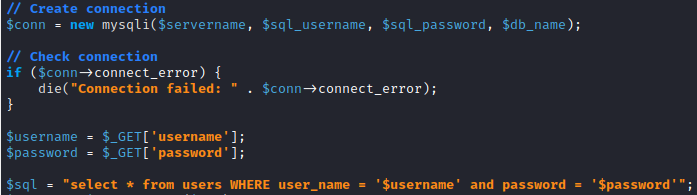
\includegraphics[width=\linewidth]{imagessqlcode/sqlcode1.png}
  \caption{Sintaxe da vuln.php}\label{fig:vuln.php}
\endminipage
\end{figure}
\begin{figure}[!htb]
\centering
\minipage{0.40\textwidth}
  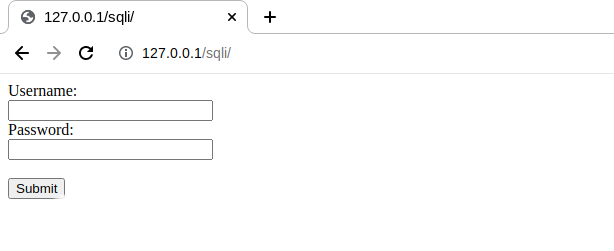
\includegraphics[width=\linewidth]{imagessql/Fig1.png}
  \caption{index.php}\label{fig:index.php}
\endminipage\hfill
\minipage{0.60\textwidth}
  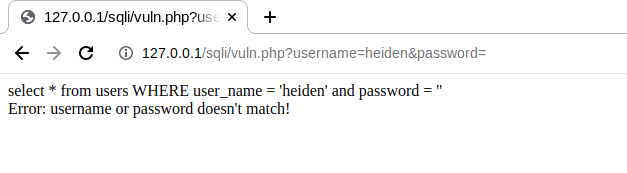
\includegraphics[width=\linewidth]{imagessql/Fig2.png}
  \caption{conta.php}\label{conta.php}
\endminipage
\end{figure}

\clearpage	
\subsection{Análise da sintaxe}

A variável \$conn vai criar uma conexão com a base de dados em que as variáveis \$servername,\$  \sql\textunderscore username, \$sql\textunderscore password e a \$db\textunderscore name armazenam, respetivamente, o ip do servidor onde esta a base de dados, o utilizador, a password e o nome da base de dados. Depois da variavel \$conn, o "if"  vai tentar se conectar com o banco de dados. Já as variaveis \$username e \$password irão receber o que o utilizador digitar.
Por último a variável \$sql seleciona tudo o que está dentro da tabela users e compara se a variável \$username está dentro da coluna user\textunderscore name e se a \$password está dentro da coluna password.

A princípio quando vamos analisar o código fonte não parece haver nada de errado mas o problema é que se o utilizador digitar comandos SQL nas variáveis \$username ou \$password estes comandos serão executados como se fizessem parte do código fonte.

\subsection{Cenário de ataque}

\subsubsection{Primeiro cenário - Bypass no sistema de login}

Vamos imaginar que o objetivo do atacante é burlar o sistema de login mesmo não sabendo qual é o utilizador ou a password que estão armazenados na base de dados. Uma das formas de burlar seria fazendo uma comparação acrescentando "' OR '1'='1'" no campo da password e colocando algo aleatório no campo do utilizador. Ao fazer isso a variável \$sql em vez de armazenar "select * from users WHERE user\textunderscore name = '\$username' and password = '\$password'" passaria a armazenar "select * from users WHERE user\textunderscore name = 'hacker' and password = '' OR '1' = '1'". Assim, mesmo que nenhum dos valores faça parte do banco de dados a variavel \$sql dará um valor True por causa do OR que acrescentamos.

\begin{figure}[!htb]
\minipage{0.40\textwidth}
  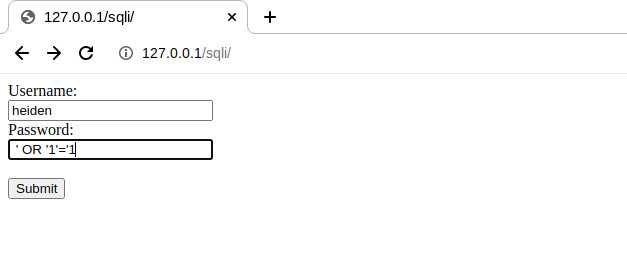
\includegraphics[width=\linewidth]{imagessql/Fig3.png}
  \caption{Ataque \ac{sqli}}\label{fig:ataque sqli}
\endminipage\hfill
\minipage{0.60\textwidth}
  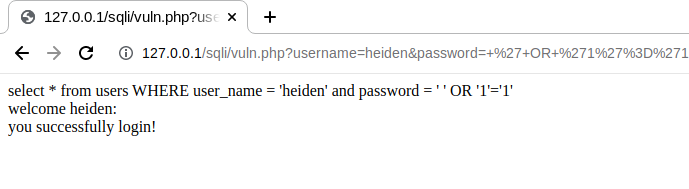
\includegraphics[width=\linewidth]{imagessql/Fig4.png}
  \caption{Resultado do ataque}\label{fig:resultado do ataque}
\endminipage
\end{figure}

Mas... E se digitarmos outras instruções SQL? Seria possível acessar o banco de dados? Para isso vamos usar uma ferramenta chamada SQLMap desenvolvida em python com o propósito de facilitar a exploração desta vulnerabilidade. 
\clearpage
\subsubsection{Segundo cenário - Acessar a base de dados}

No início deste capítulo dissemos que uma das consequências do \ac{sqli} é o acesso direto a tudo o que está dentro de uma base de dados mas, para facilitar a exploração desta vulnerabilidade vamos usar o SQLMap que vai nos ajudar no processo.\cite{sqlmapproject}

O primeiro comando que digitamos para iniciar o ataque, python3 sqlmap.py -u 'http://127.0.0.1/vuln.php?username=andre\&password=p4ssw0rd' --dbs, tem como finalidade testar varias instruções SQL para depois extrair as bases de dados presentes no servidor. O parâmetro -u exige que seja colocada a URL entre aspas junto com os parametros do servidor que são vulneráveis a SQLI (ou seja, o parâmetro username e o parâmetro password) enquanto o parâmetro --dbs exige que seja extraída o nome das bases de dados.
\begin{figure}[h]
 \centering
 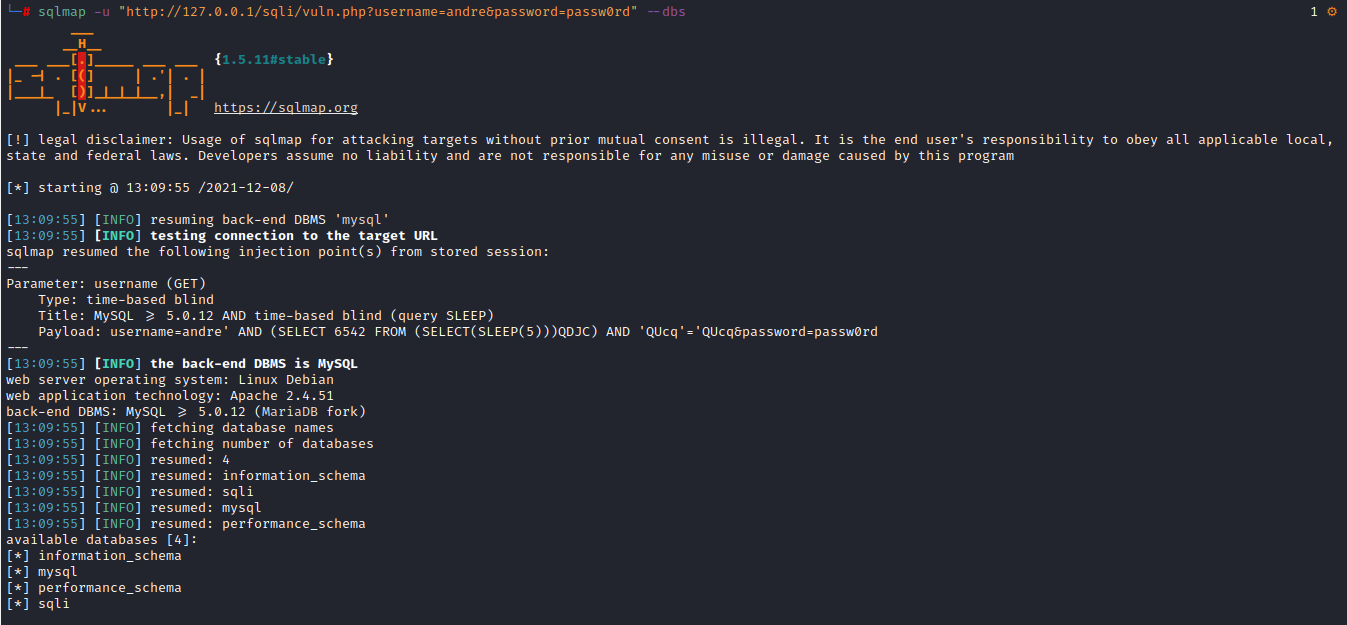
\includegraphics[scale=0.25]{imagessql/Fig5.png}
 \caption{Extração de base de dados}
\end{figure}  


Como podemos ver o SQLMap encontrou quatro bases de dados. As três primeiras são bases de dados que fazem parte do MySQL, já a ultima é aquela que vamos analisar mais a fundo para encontrar o usuário e a senha que precisamos. Agora em vez de colocarmos --dbs no final, vamos substituir pelo parâmetro -D onde iremos colocar o nome base de dados que queremos extrair e por ultimo o parâmetro --dump que irá comunicar ao sqlmap para extrair tudo o que está dentro da base de dados.
\clearpage
\begin{figure}[h]
 \centering
 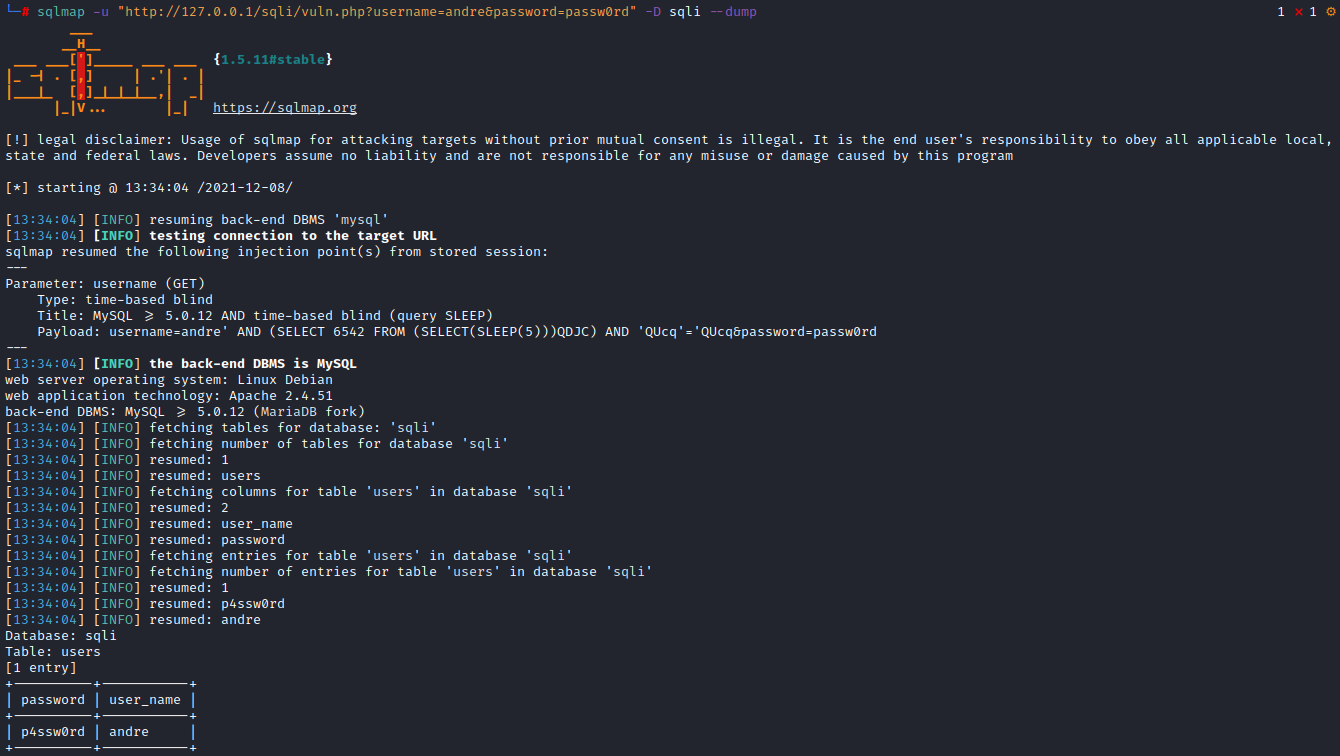
\includegraphics[scale=0.27]{imagessql/Fig6.png}
 \caption{Extração da base de dados}\label{extração da base de dados}
\end{figure}  

O SQLMap encontrou dentro da base de dados uma tabela chamada "users", duas colunas chamadas "user\textunderscore name" e "password" e dentro delas estão o usuário e a senha que procurávamos! Por último vamos testar se realmente estes são o utilizador e a password que precisávamos.


\begin{figure}[h]
 \centering
 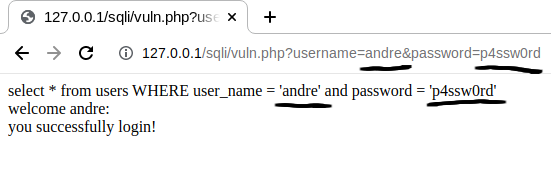
\includegraphics[scale=0.7]{imagessql/Fig7.png}
 \caption{Teste das credenciais}\label{teste das credenciais}
\end{figure}  
\clearpage

\subsection{Como prevenir}

Existem várias formas de prevenir o \ac{sqli} mas a mais comum seria filtrando os caracteres digitados pelo utilizador. Uma das possíveis soluções seria criar um array e depois filtrar as instruções SQL. Outra solução possível seria usar uma das funções presentes no PHP para filtrar o que o utilizador digita, por exemplo a mysqli\textreal \textunderscore real \textunderscore escape\textunderscore string() que irá colocar "/" entre os caracteres especiais usados nas instruções SQL. Para aplicar a função só temos que colocar dentro dela a variável \$conn e depois a variável que armazena o que o utilizador digitou e assim resolvemos o problema.

\begin{figure}[h]
 \centering
 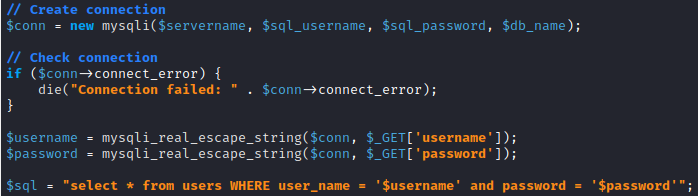
\includegraphics[scale=0.5]{imagessqlcode/sqlcode2.png}
 \caption{Sintaxe vuln.php}\label{sintaxe vuln.php}
\end{figure}


\begin{figure}[h]
 \centering
 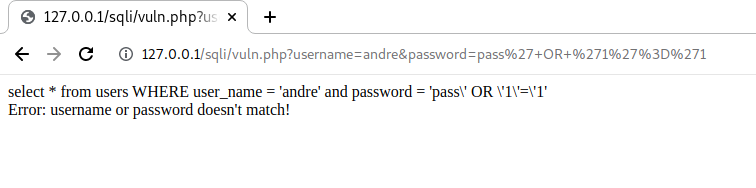
\includegraphics[scale=0.5]{imagessql/Fig8.png}
 \caption{vuln.php}\label{vuln.php}
\end{figure}  

\clearpage	
\section{Cross-site Scripting}
\subsection{Descrição geral e consequências}

O \ac{xss} é uma vulnerabilidade que permite ao atacante injetar scripts em javascript ou até mesmo instruções em HTML ou XML de forma a tirar proveito dos utilizadores. Esta vulnerabilidade consegue ser mais frequente do que o \ac{sqli}, tendo sido encontrada por hackers portugueses nos sites da CIA, FBI, NASA e no Departamento de Estado dos EUA. Existem três variantes de ataques \ac{xss}: Reflected XSS, Stored XSS e o DOM XSS. 

O Reflected XSS é um ataque em que se injeta o script diretamente na URL e a página executa o que foi introduzido, mas este não fica armazenado no servidor o que implica que o mesmo tenha que enviar a URL para as vítimas de forma a obter proveito delas. 

O Stored XSS é um ataque em que o script é injetado na página fazendo com que qualquer um que entre na mesma fique comprometido pois, ao contrário do anterior, este fica armazenado no servidor sendo o ataque XSS mais perigoso já catalogado.

Por último o DOM XSS que é uma variante do Reflected XSS e por isso não nos vamos estender sobre.
\cite{cia-nasa}	
\clearpage
\subsection{Código exemplo}

 No index.php decidimos criar duas opções. Na primeira opção o utilizador pode escrever alguma coisa que será exibida na vuln.php sem armazenar o que foi digitado. Já na segunda opção o utilizador pode fazer um comentário que será guardado num arquivo chamado comentario.html e depois será exibido em vuln.php, lembrando que ambas as opções usam o método GET.
Agora vamos analisar uma parte do código do arquivo vuln.php:

\begin{figure}[!htb]
\centering
\minipage{0.6\textwidth}
  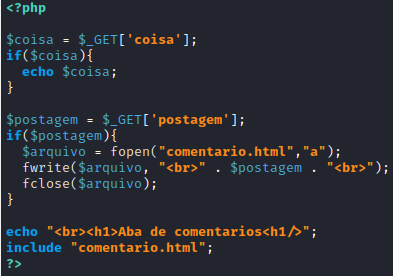
\includegraphics[width=\linewidth]{imagessqlcode/sqlcode3.png}
  \caption{Sintaxe do vuln.php}\label{sintaxe vuln.php}
\endminipage
\end{figure}
\begin{figure}[!htb]
\minipage{0.33\textwidth}
  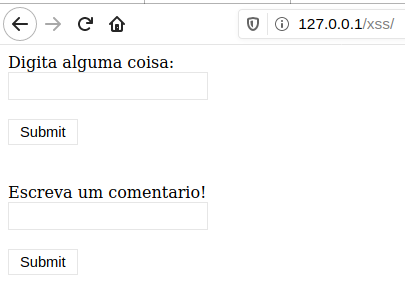
\includegraphics[width=\linewidth]{imagessql/Fig9.png}
  \caption{index.php}\label{index.php}
\endminipage\hfill
\minipage{0.33\textwidth}
  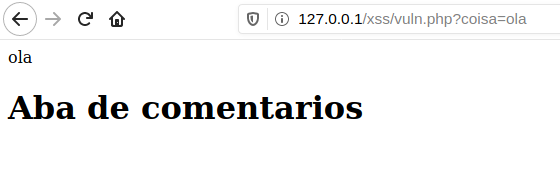
\includegraphics[width=\linewidth]{imagessql/Fig10.png}
  \caption{vuln.php}\label{vuln.php}
\endminipage
\end{figure}
\clearpage
\subsection{Análise da sintaxe}

A variável \$coisa armazena o que foi digitado na primeira opção e depois é exibida quando o "if" é executado. Já a variável \$postagem armazena o que foi digitado na segunda opção e quando o "if" é executado a variável \$arquivo abre o comentario.html. Quando o arquivo é aberto o fwrite escreve uma linha com o que está dentro da variável \$postagem e coloca no início e no fim o  <br> que serve para mudar de linha. Quando a linha é adicionada o arquivo é fechado através do comando fclose e depois é apresentado através do include.

Tal como no \ac{sqli}, a princípio não parece haver nada de errado com o código mas o problema é que a informação não é filtrada e por isso se digitarmos instruções em HTML ou em javascript estas serão executadas.

\subsection{Cenário de ataque}

\subsubsection{Primeiro cenário - Reflected XSS}

Vamos imaginar que o atacante está há procura de uma vulnerabilidade XSS no servidor e começa por testar a primeira opção. Para isso ele acrescenta uma instrução em javascript no campo de texto, por exemplo <script>alert("aqui existe xss")</script>.

\begin{figure}[!htb]
\minipage{0.450\textwidth}
  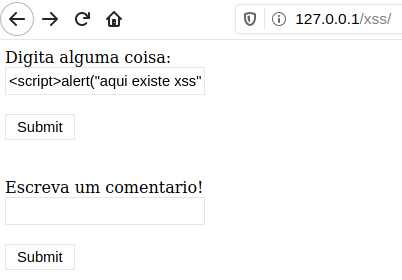
\includegraphics[width=\linewidth]{imagessql/Fig11.png}
  \caption{XSS no primeiro campo}\label{XSS no primeiro campo}
\endminipage\hfill
\minipage{0.450\textwidth}
  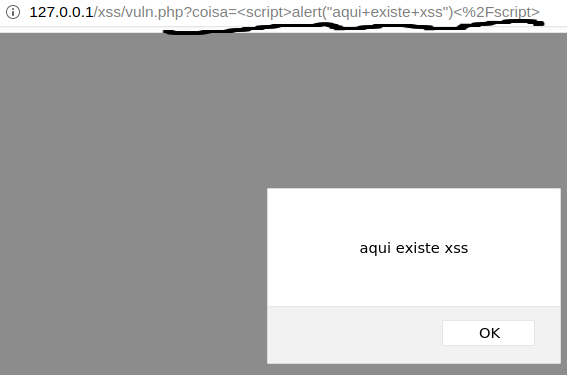
\includegraphics[width=\linewidth]{imagessql/Fig12.png}
  \caption{Resultado}\label{fig:resultado}
\endminipage
\end{figure}

Como podemos ver, a instrução foi executada pelo sistema, o que significa que se enviarmos para alguém a URL com a instrução que colocamos a mesma será executada. Agora pensem na quantidade de opções que um possível atacante pode pensar para extrair informações das vítimas através de um site legitimo, sem contar que o servidor não tem como saber se o ataque foi feito devido ao facto de não armazenar as informações digitadas.
\clearpage
\subsubsection{Segundo cenário - Stored XSS}

O atacante com o mesmo propósito que no cenário anterior em vez de testar a primeira opção irá testar a segunda, mas usando a mesma instrução para testar se é vulnerável a XSS. A diferença de um cenário para outro é que neste a informação digitada fica armazenada no servidor o que faz com que qualquer um que entre na página tenha o script executado no seu navegador.

\begin{figure}[!htb]
\minipage{0.50\textwidth}
  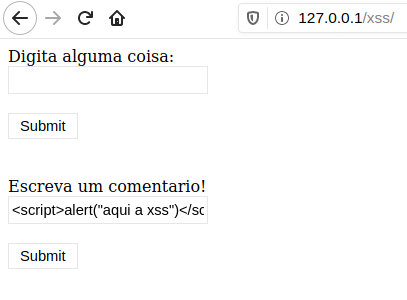
\includegraphics[width=\linewidth]{imagessql/Fig13.png}
  \caption{XSS no segundo campo}\label{XSS no segundo campo}
\endminipage\hfill
\minipage{0.50\textwidth}
  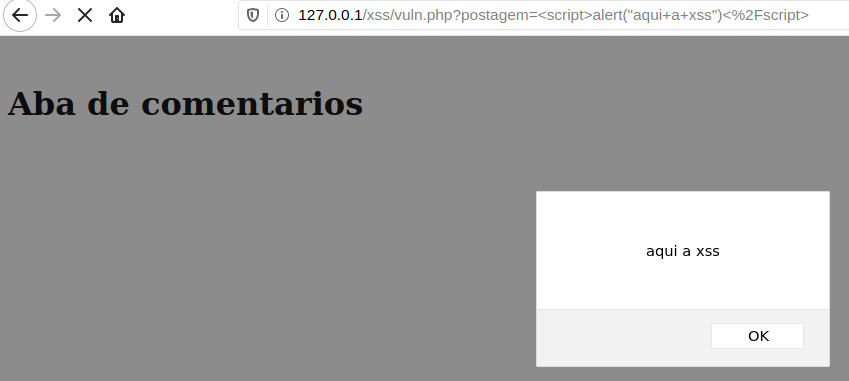
\includegraphics[width=\linewidth]{imagessql/Fig14.png}
  \caption{Resultado}\label{Resultado}
\endminipage
\end{figure}

\begin{figure}[h]
 \centering
 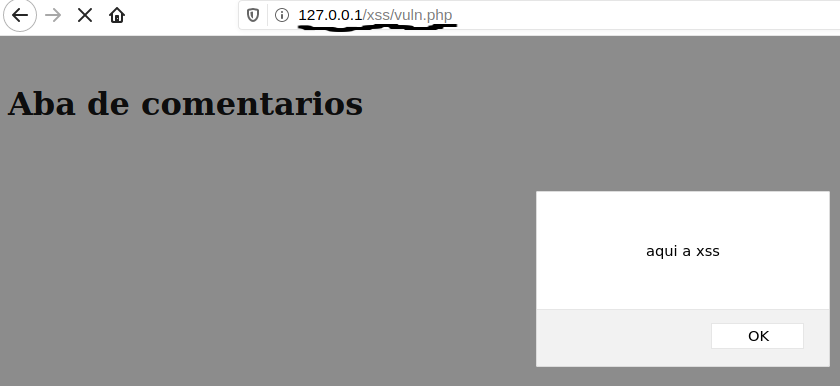
\includegraphics[scale=0.3]{imagessql/Fig15.png}
 \caption{Stored XSS}\label{Stored XSS}
\end{figure}
\clearpage

\subsection{Como prevenir}

Nos cenários de ataque que apresentamos, podemos concluir que esta vulnerabilidade afeta o servidor mas afeta mais quem o acessa. As soluções usadas para corrigir o XSS são idênticas aos métodos usados para corrigir o SQLI. A mais geral seria filtrar as instruções mas uma boa opção seria usar a função htmlspecialchars() que converte os caracteres em entidades HTML impossibilitando assim a execução das instruções.

\begin{figure}[!htb]
\minipage{0.4\textwidth}
  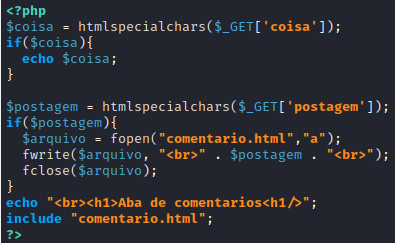
\includegraphics[width=\linewidth]{imagessqlcode/sqlcode4.png}
  \caption{Sintaxe vuln.php}\label{Sintaxe vuln.php}
\endminipage\hfill
\minipage{0.60\textwidth}
  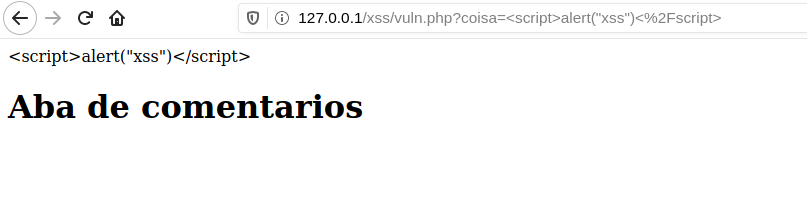
\includegraphics[width=\linewidth]{imagessql/Fig16.png}
  \caption{Primeiro campo}\label{Primeiro campo}
\endminipage
\end{figure}

\begin{figure}[!htb]
\minipage{0.4\textwidth}
  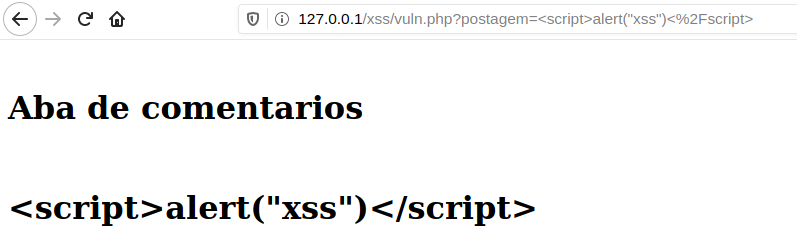
\includegraphics[width=\linewidth]{imagessql/Fig17.png}
  \caption{Segundo campo}\label{Segundo campo}
\endminipage\hfill
\minipage{0.6\textwidth}
  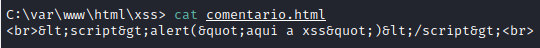
\includegraphics[width=\linewidth]{imagessql/Fig18.png}
  \caption{Output do comentario.html}\label{Output do comentario.html}
\endminipage
\end{figure}


\clearpage
\section{OS Command Injection}


\subsection{Descrição geral e consequências}

O OS Command Injection é uma vulnerabilidade que permite ao atacante executar comandos no OS do servidor. Esta vulnerabilidade muito recorrente acontece pela falta de verificação do que é introduzido, passando essa informação digitada para uma shell do OS. Podemos considerar esta vulnerabilidade como uma das mais perigosas já catalogadas na história da cibersegurança porque quem explora a mesma tem os seus comandos executados com as permissões da aplicação vulnerável em que na maioria dos casos o invasor pode ver o que está dentro dos arquivos do servidor, editar os mesmos, fazer upload de arquivos, executar backdoors, etc tornando-a assim numa das mais temidas.

\clearpage
\subsection{Código exemplo}

Para ilustrar a vulnerabilidade decidimos criar uma página chamada index.php onde o utilizador pode colocar um site que depois de ser submetido será enviado através do parâmetro server para outra pagina chamada ping.php que irá testar se o servidor está no ar ou não, lembrando que nesta situação o parâmetro "server" envia a informação através do método GET.

\begin{figure}[!htb]
\minipage{0.40\textwidth}
  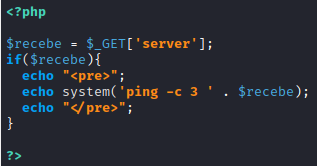
\includegraphics[width=\linewidth]{imagessqlcode/sqlicode5.png}
  \caption{Sintaxe ping.php}\label{ping.php}
\endminipage\hfill
\minipage{0.40\textwidth}
  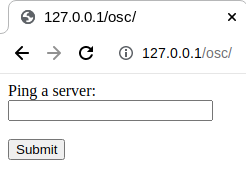
\includegraphics[width=\linewidth]{imagessql/Fig19.png}
  \caption{index.php}\label{index.php}
\endminipage
\end{figure}

\begin{figure}[!htb]
\minipage{1.0\textwidth}
  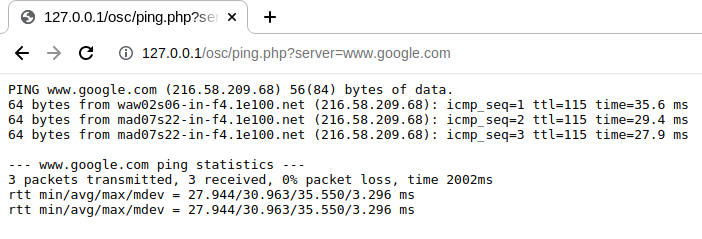
\includegraphics[width=\linewidth]{imagessql/Fig20.png}
  \caption{ping.php}\label{ping.php}
\endminipage
\end{figure}
\clearpage
\subsection{Análise da sintaxe}

A informação enviada através do parâmetro server será armazenada numa variável chamada \$recebe. Quando o "if" é executado, as instruções echo escrevem <pre> que tem como objetivo formatar o texto que está depois dela. Dentro destas instruções existe outro echo que executa a função system() que tem como objetivo executar o comando "ping -c 3 " junto com a variavél \$recebe numa shell do OS do servidor, verificando assim se o servidor digitado está no ar ou não.

\subsection{Cenário de ataque}

Vamos supor que o atacante tem como objetivo enviar uma backdoor para dentro do servidor e depois executa-la para ter acesso a tudo. Uma das formas de o fazer seria digitando o site que se pretende ver se está no ar ou não, seguido de "\&\&" para escrever outro comando a seguir e depois colocando o comando que se pretende. Vamos supor que ele usa o comando wget para baixar a backdoor, (back.php.txt), para dentro do servidor, (back.php), seguido do comando ls para visualizar os arquivos que estão dentro da pasta.
\begin{figure}[h]
 \centering
 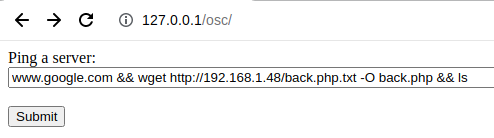
\includegraphics[scale=0.3]{imagessql/Fig21.png}
 \caption{Intrução maliciosa}\label{instrução maliciosa}
\end{figure}

\begin{figure}[h]
 \centering
 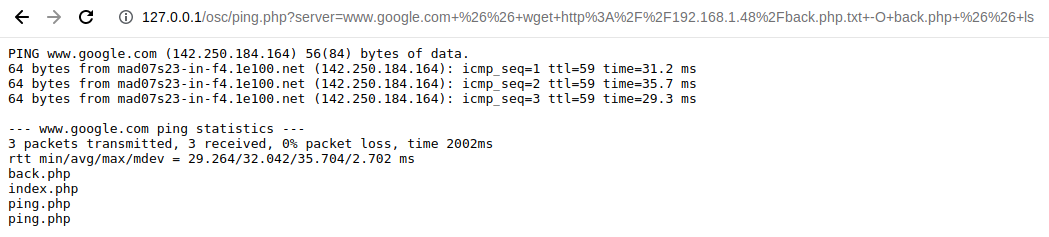
\includegraphics[scale=0.3]{imagessql/Fig22.png}
 \caption{Resultado}\label{resultado}
\end{figure}
Como podemos ver a backdoor cujo nome é back.php foi enviada para o servidor com sucesso! Agora vamos executar a backdoor usando o comando "php back.php" para ver se conseguimos obter acesso ao servidor.
\clearpage
\begin{figure}[h]
 \centering
 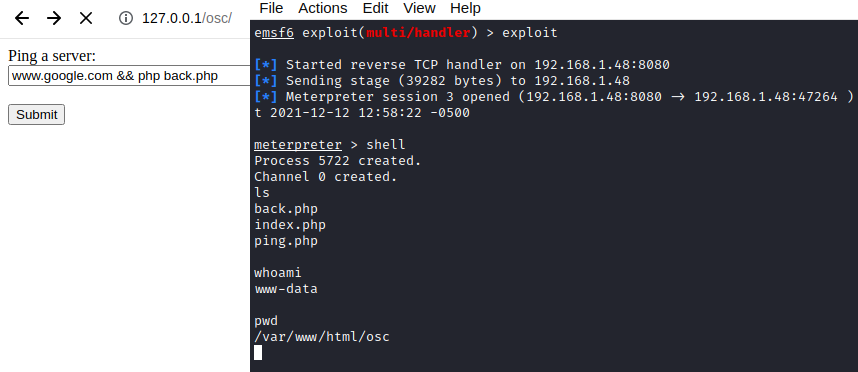
\includegraphics[scale=0.4]{imagessql/Fig23.png}
 \caption{Meterpreter}\label{meterpreter}
\end{figure}

Como podemos ver a backdoor foi executada com sucesso, depois de esta ser executada ainda testamos os comandos ls, whoami e pwd que foram executados sem quaisquer problemas. A conclusão que podemos tirar deste ataque é que apenas com dois comandos nós conseguimos colocar uma backdoor e executa-la o que comprova o quão perigosa é esta vulnerabilidade devido há liberdade que dá ao atacante para ele fazer o que bem entende do servidor.

\clearpage
\subsection{Como prevenir}

Existem algumas formas de corrigir esta vulnerabilidade, como por exemplo filtrando os caracteres "&&", ";", etc mas este método não é perfeito pois existem outros tipos de caracteres que podem ser usados e que podemos nos esquecer de filtrar. O método mais recomendado seria evitar usar funções que executem comandos no OS e substitui-las por outras funções que foram desenhadas para fazer o que precisamos sem ter que executar comandos. Por exemplo neste caso nós vamos usar uma função chamada gethostbyname() que irá converter o servidor digitado em um ip caso o mesmo esteja no ar, caso não esteja no ar a função não irá fazer essa conversão.

\begin{figure}[!htb]
\minipage{0.50\textwidth}
  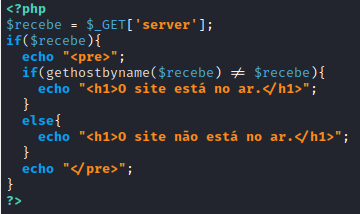
\includegraphics[width=\linewidth]{imagessqlcode/sqlicode6.png}
  \caption{ping.php}\label{ping.php}
\endminipage\hfill
\minipage{0.50\textwidth}
  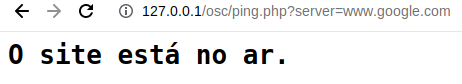
\includegraphics[width=\linewidth]{imagessql/Fig24.png}
  \caption{Teste sem injeção}\label{teste sem injeção}
\endminipage
\end{figure}

\begin{figure}[h]
 \centering
 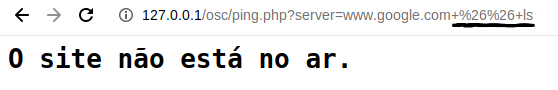
\includegraphics[scale=0.3]{imagessql/Fig25.png}
 \caption{Teste com injeção}\label{teste sem injeção}
\end{figure}

























\chapter{Conclusões}
\label{chap.conclusao}
Neste trabalho discutimos algumas vulnerabilidades web, foi elaborada uma contextualização de modo a que essas vulnerabilidades sejam reconhecidas e evitadas mais facilmente pelos utilizadores.
Tendo em conta o exposto consideramos que as vulnerabilidades estão cada vez mais presentes no nosso dia a dia  e por isso deve existir uma conduta responsável e atenta no uso das  ferramentas web.
Assim, com a finalização do trabalho recomendamos a que o leitor se informe sobre mais vulnerabilidades web, e que procure sempre aprender para bem da sua segurança.
\cite{owasptop10}

\chapter*{Contribuições dos autores}
O autor AM ficou encarregue do capitulo Broken Access Control, e o autor AC ficou encarregue do capitulo de Injeção.
O restante do trabalho foi executado pelos 2 autores, tendo sido a percentagem de contribuição de cada um 50\%.


%%%%%%%%%%%%%%%%%%%%%%%%%%%%%%%%%
\chapter*{Acrónimos}
\begin{acronym}
\acro{ua}[UA]{Universidade de Aveiro}
\acro{lei}[LEI]{Licenciatura em Engenharia Informática}
\acro{bac}[BAC]{Broken Access Control}
\acro{lfi}[LFI]{Local File Inclusion}
\acro{jwt}[JWT]{JSON Web Token}
\acro{sqli}[SQLI]{SQL Injection}
\acro{xss}[XSS]{Cross-site Scripting}
\end{acronym}


%%%%%%%%%%%%%%%%%%%%%%%%%%%%%%%%%
\printbibliography

\end{document}
